\subsubsection{Variant Filtering}

%TODO: For HaplotypeCaller we should check if splitting snps/indels sites into snps and indels yield a greater SNP accuracy rather than salvaging the SNPs from the INDEL-filtered snps/indels sites. Perhaps call SNP and BOTH separately...

Filtering will be carried out with GATK3.4 \gls{VR}. GATK best practices will be used for filtering SNPs.
%http://gatkforums.broadinstitute.org/discussion/1259/which-training-sets-arguments-should-i-use-for-running-vqsr
We will use HapMap III and 1000G phase 1 Omni2.5 sites as truth and training sets (prior probabilities of 15 and 12). High confidence 1000G phase 1 SNPs will be used as an additional training set (prior 10). This dataset does not contain Y chromosome variants. %For indels we will use the Mills and Devine and 1000G gold standard as a truth and training set (prior 12). In both cases
dbSNP138 or newer will act as a set of known sites.
To build our Gaussian mixture model we use annotations at each site related to coverage (QD=QualByDepth and DP), strand bias (FS=FisherStrand, SOR=StrandOddsRatio), mapping quality (MQ, MQRankSum, ReadPosRankSum).
%For indels we use the same annotations, except for MQ being left out.
DP is the approximate read depth after filtering reads with poor mapping quality and bad mates. QD is the variant confidence normalized by the unfiltered depth for the variant allele. FS is a Phred-scaled p-value using Fisher's exact test to detect strand bias. SOR is the odds ratio of a 2x2 contingency table (rows and columns are positive/negative strand and reference/alternate allele) to detect strand bias. MQ is the RMS of the mapping qualities, which serves an an average across reads and samples. MQRankSum is the Z-score from a Wilcoxon rank sum test of alternate vs. reference mapping qualities. ReadPosRankSum is the Z-score from a Wilcoxon rank sum test of alternate vs. reference read position biases.
%When not doing variant calling with HaplotypeCaller we
We will also use the annotation HaplotypeScore, which is a statistical measure of more than 2 haplotypes being present at the same site for a sample.

The NA12878 sample will be included at an appropriate coverage, when doing variant calling. PCR-free reads will be used for the validation sample to avoid PCR artefacts. The inclusion of NA12878 allows for selection of a filtering threshold, which yields a good balance between sensitivity and specificity after filtering. Specifically ROC curves will be generated for sample NA12878, for which highly curated SNPs
%and short INDELs
are available for chromosomes 1-22 and X. The ROC curves will be sorted by the variant quality score log odds ratios calculated by VariantRecalibrator.
%For structural variants we will use PacBio 54x NA12878 WGS data as a truth set. %ftp://ftp.1000genomes.ebi.ac.uk/vol1/ftp/technical/working/20131209_na12878_pacbio/si/

%For cohorts with 10 or more founder samples the InbreedingCoeff annotation will also be used. It is a likelihood-based Hardy-Weinberg test for the inbreeding among samples. It will be tested by generation of additional ROC curves, whether the inclusion of the InbreedingCoeff annotation worsens the ability to do VQSR correctly, when there are many related samples. Whenever available pedigree information will be used during variant calling to assist in the calculation of the InbreedingCoeff annotation.

%We apply the filtering by doing a binary heap merge of unfiltered variants to 1) allow two VQSR processes to run simultaneously; i.e. one for SNPs and one for indels and to 2) avoid lexicographical sorting of already numerically sorted files (i.e. VCF and recal files are sorted numerically by genomic coordinate). Alternatively one can run GATK VariantRecalibrator and ApplyRecalibration in sequence twice, which is twice as slow. Furthermore the heap merge only requires a line from the SNP .recal file, the INDEL .recal file and the VCF file to be held in memory at once.
%The excludemarkers option of the current release of Beagle4 cannot be used to apply the filtering, because 1) UG emits two separate VCF records for SNPs and indels at the same site and 2) the excludemarkers option of Beagle4 only allows one to specify variants by rsID or genomic coordinate. The excludemarkers option would otherwise save disk space and time.

Unlike \gls{1000G} phase 1 and \gls{GoNL} we will not filter out multiallelic variants, because we don't find them to be of lower quality than biallelic SNPs and because there is a greater probability of these appearing across thousands of samples from multiple populations from the African continent than in hundreds of samples from one European country. For example 1 in every \~50 SNP in ~2000 Ugandan samples sequenced to a depth of 4x is multiallelic.
%They probably did this, because Beagle3 didn't support multiallelic variants...

\gls{VR} will be applied separately for the autosomes and the X chromsome, because we have shown \gls{VR} culprits to be different for the autosomes and the X chromosome \ref{fig:VRculprits}, because their depth of coverage and hence their depth derived annotations are different.

\begin{figure}[!htbp]
\centering
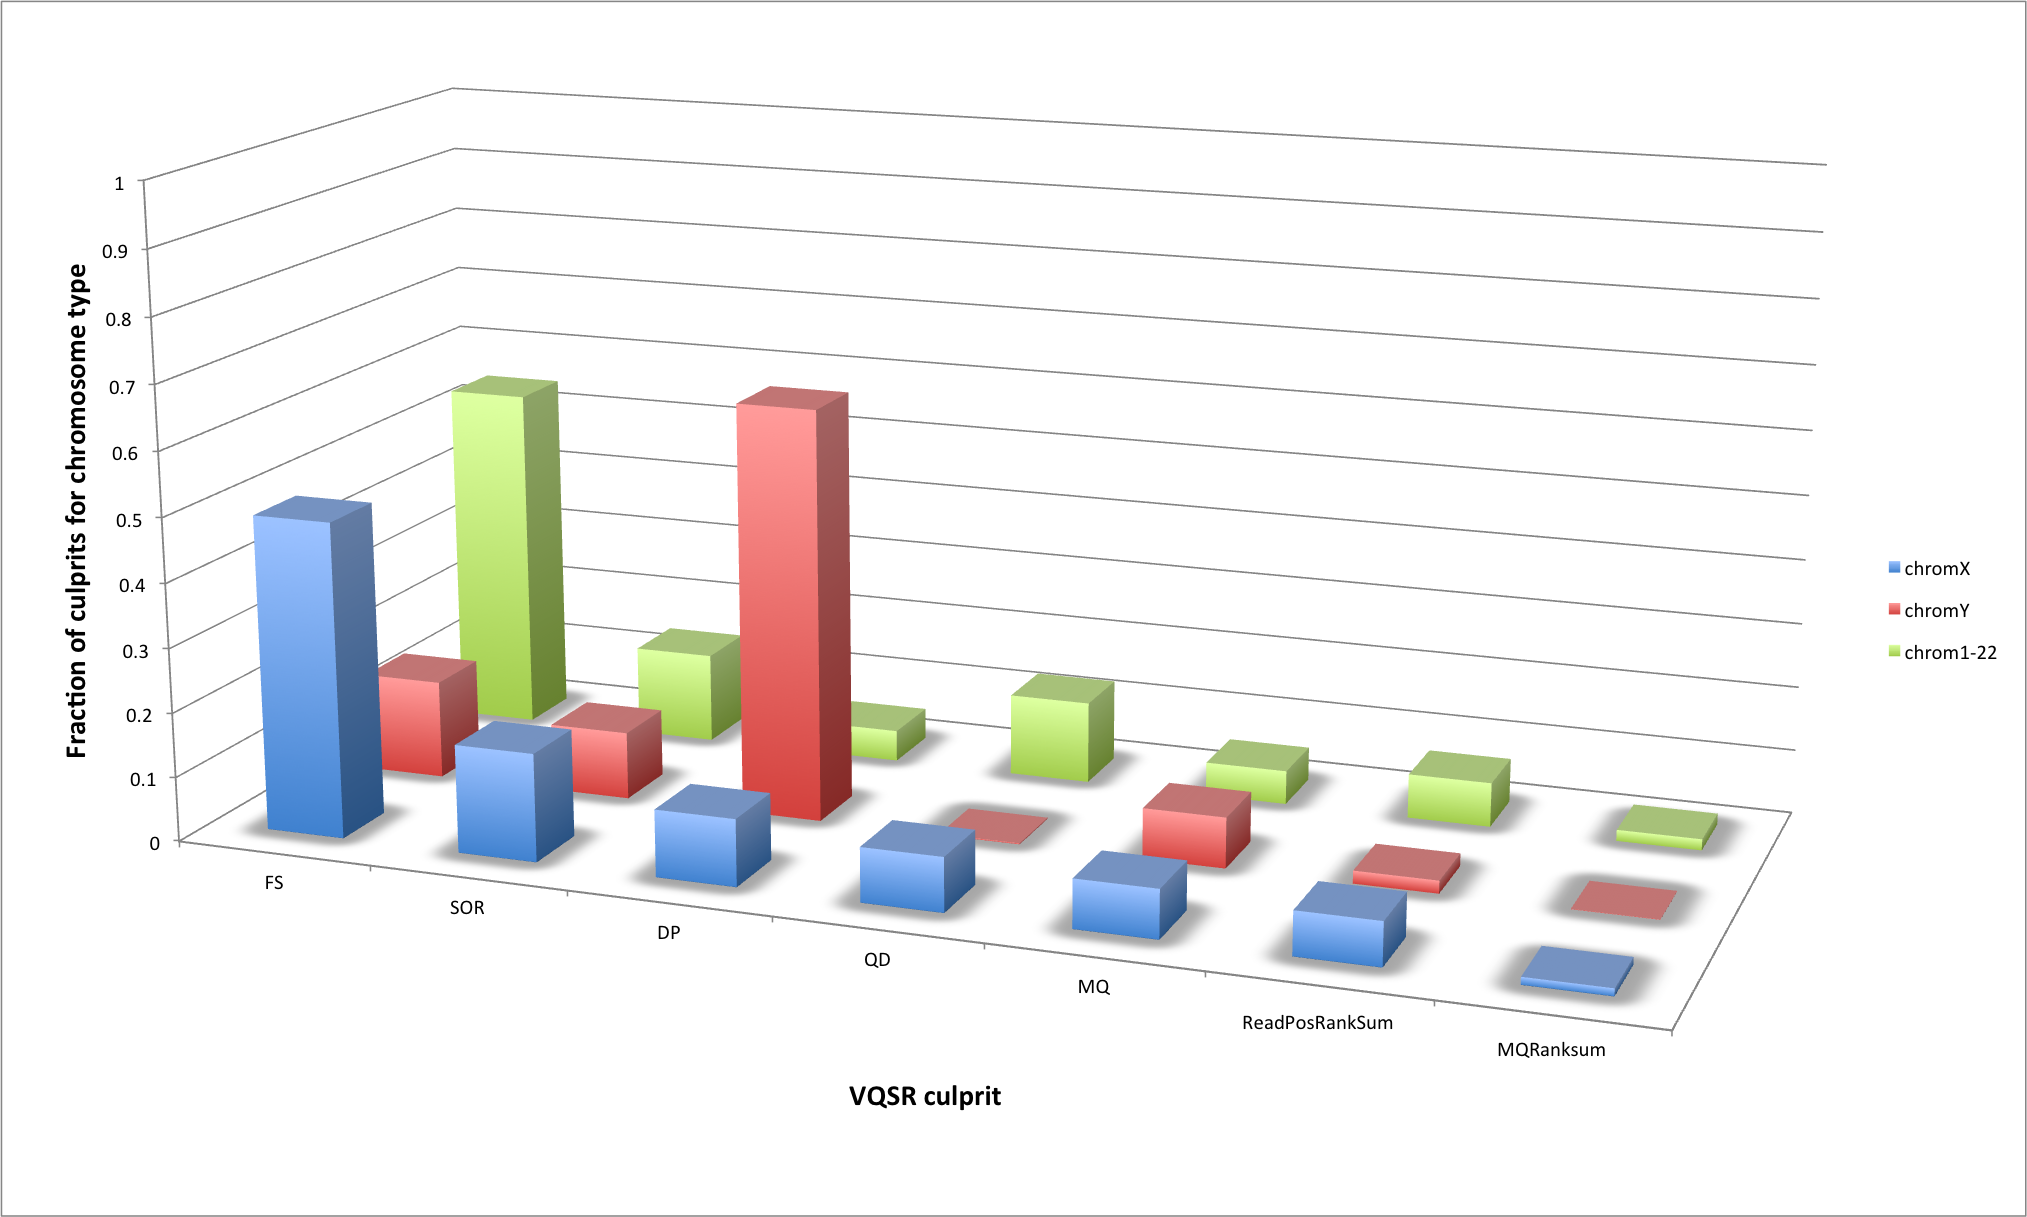
\includegraphics[width=0.8\textwidth]{VRculprits}
\caption[Distribution of variant filtering culprits for the autosomes and sex chromosomes.]{The autosomes and sex chromosomes have different depths of coverage, because only one copy of the non-\gls{PAR} Some of the annotations used by \gls{GATK} \gls{VR} are depth dependent. This figure shows the normalised frequency distribution of culprits as determined by \gls{VR}.}
\label{fig:VRculprits}
\end{figure}

The SNP count after variant filtering is summarised in table \ref{tab:SNPcount}.

\begin{figure}[!htbp]
\centering
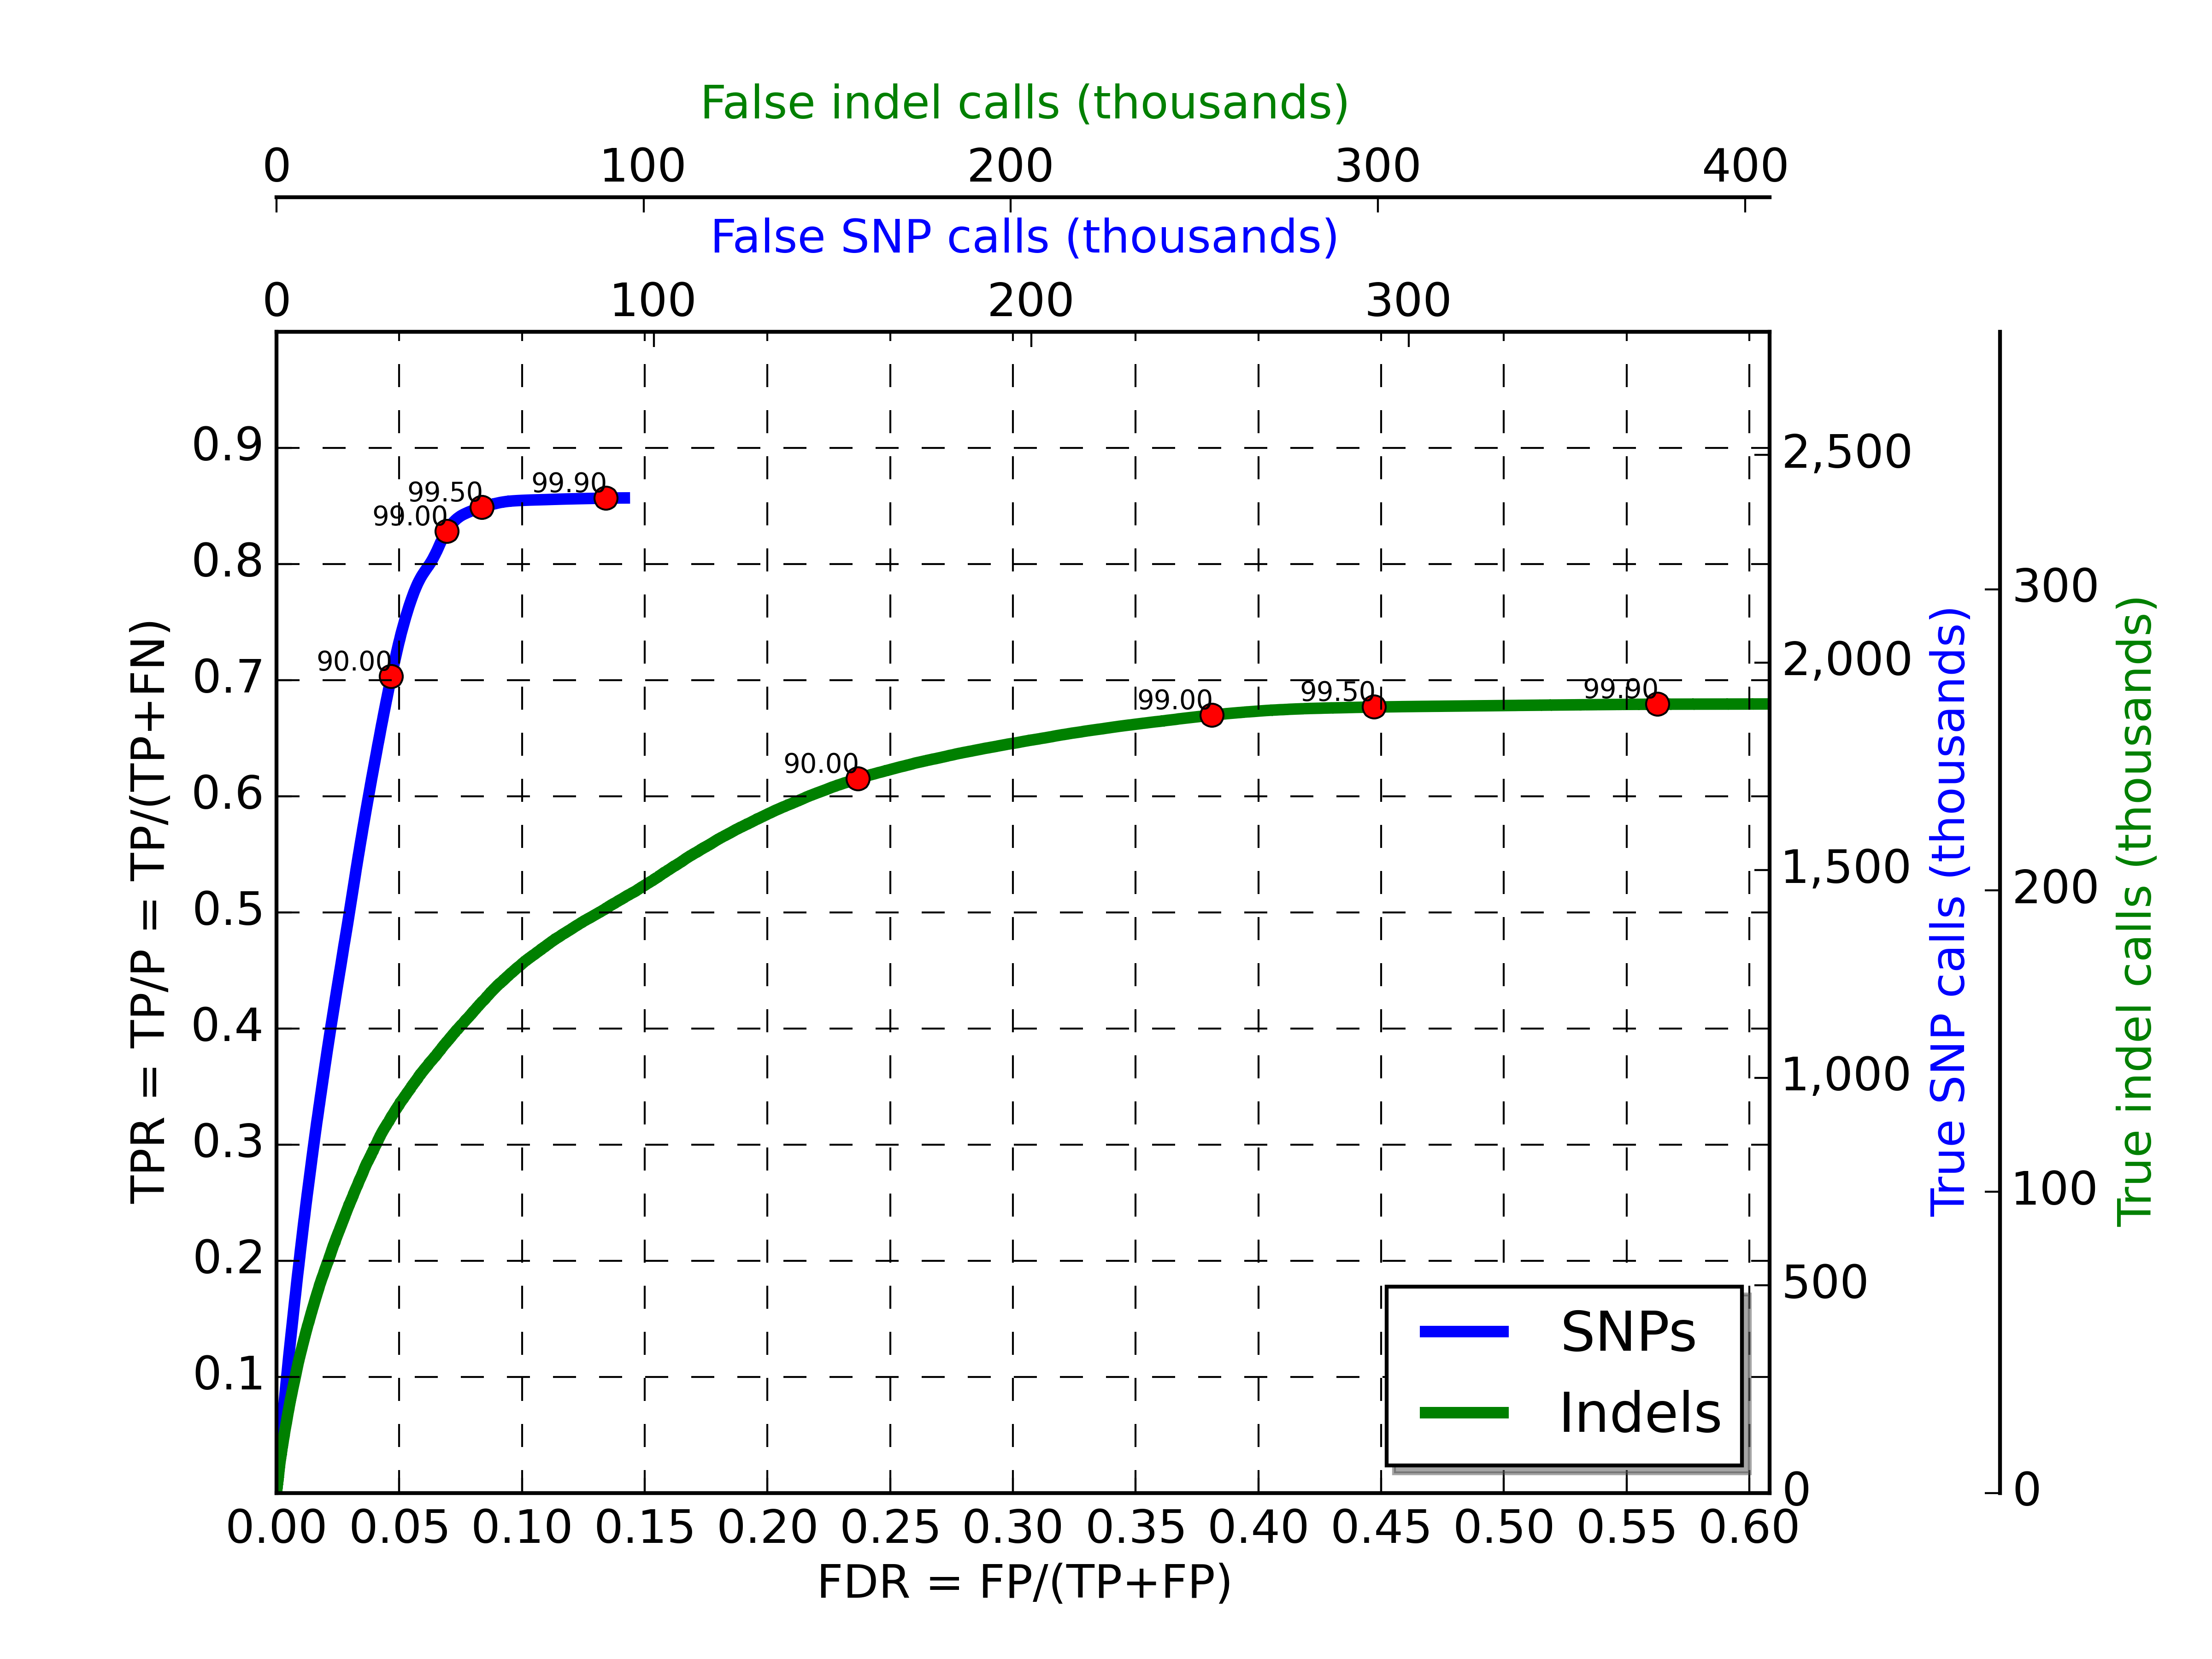
\includegraphics[width=0.8\textwidth]{FDR_ADRP_UG34}
\caption[ROC curve for SNPs and indels.]{We used sample NA12878 for which a gold standard truth set is available to calculate sensitivity and specificity as a function of VQSLOD. We use the plot to select the optimal truth sensitivity threshold. This plot is for calls on the \gls{ADRP} samples using \gls{GATK} \gls{UG} 3.4}
\label{fig:ROC1}
\end{figure}